\documentclass[a4paper]{article}

\input{style/ch_xelatex.tex}
\input{style/scala.tex}

\graphicspath{ {images/} }
\usepackage{ctex}
\usepackage{graphicx}
\usepackage{color,framed}%文本框
\usepackage{listings}
\usepackage{caption}
\usepackage{tcolorbox}
\usepackage{hyperref}
\hypersetup{hidelinks,
	colorlinks=true,
	allcolors=black,
	pdfstartview=Fit,
	breaklinks=true}

\usepackage{amssymb}
\usepackage{enumerate}
\usepackage{xcolor}
\usepackage{bm} 
\usepackage{lastpage}%获得总页数
\usepackage{fancyhdr}
\usepackage{tabularx}  
\usepackage{geometry}
\usepackage{minted}
\usepackage{graphics}
\usepackage{subfigure}
\usepackage{float}
\usepackage{pdfpages}
\usepackage{pgfplots}
\pgfplotsset{width=10cm,compat=1.18}
\usepackage{multirow}
\usepackage{footnote}
\usepackage{booktabs}
\usepackage{listings}
\captionsetup{font=small, labelfont=bf, skip=6pt}

%-----------------------伪代码------------------
\usepackage{algorithm}  
\usepackage{algorithmicx}  
\usepackage{algpseudocode}  
\floatname{algorithm}{Algorithm}  
\renewcommand{\algorithmicrequire}{\textbf{Input:}}  
\renewcommand{\algorithmicensure}{\textbf{Output:}} 
\usepackage{lipsum}  
\makeatletter
\newenvironment{breakablealgorithm}
  {% \begin{breakablealgorithm}
  \begin{center}
     \refstepcounter{algorithm}% New algorithm
     \hrule height.8pt depth0pt \kern2pt% \@fs@pre for \@fs@ruled
     \renewcommand{\caption}[2][\relax]{% Make a new \caption
      {\raggedright\textbf{\ALG@name~\thealgorithm} ##2\par}%
      \ifx\relax##1\relax % #1 is \relax
         \addcontentsline{loa}{algorithm}{\protect\numberline{\thealgorithm}##2}%
      \else % #1 is not \relax
         \addcontentsline{loa}{algorithm}{\protect\numberline{\thealgorithm}##1}%
      \fi
      \kern2pt\hrule\kern2pt
     }
  }{% \end{breakablealgorithm}
     \kern2pt\hrule\relax% \@fs@post for \@fs@ruled
  \end{center}
  }
\makeatother
%------------------------代码-------------------
\RequirePackage{listings}
\RequirePackage{xcolor}
\definecolor{dkgreen}{rgb}{0,0.6,0}
\definecolor{gray}{rgb}{0.5,0.5,0.5}
\definecolor{mauve}{rgb}{0.58,0,0.82}
\lstset{
	numbers=left,  
	frame=tb,
	aboveskip=3mm,
	belowskip=3mm,
	showstringspaces=false,
	columns=flexible,
	framerule=1pt,
	rulecolor=\color{gray!35},
	backgroundcolor=\color{gray!5},
	basicstyle={\ttfamily},
	numberstyle=\tiny\color{gray},
	keywordstyle=\color{blue},
	commentstyle=\color{dkgreen},
	stringstyle=\color{mauve},
	breaklines=true,
	breakatwhitespace=true,
	tabsize=3,
}

%-------------------------页面边距--------------
\geometry{a4paper,left=2.3cm,right=2.3cm,top=2.7cm,bottom=2.7cm}
%-------------------------页眉页脚--------------
\usepackage{fancyhdr}
\pagestyle{fancy}
\lhead{\kaishu 计算机系统前沿}% @这里是填写什么名字的实验报告
\chead{存储设备性能测试和分析} % 这里是填写本次实验的名字
\rhead{2312966 {\CJKfontspec{simkai.ttf} 林晖鹏}}%加粗\bfseries 
\lfoot{}
\cfoot{\thepage}
\rfoot{}
\renewcommand{\headrulewidth}{0.1pt}  
\renewcommand{\footrulewidth}{0pt}%去掉横线
\newcommand{\HRule}{\rule{\linewidth}{0.5mm}}%标题横线
\newcommand{\HRulegrossa}{\rule{\linewidth}{1.2mm}}
\setlength{\textfloatsep}{10mm}%设置图片的前后间距
%--------------------文档内容--------------------

\begin{document}
\renewcommand{\contentsname}{目\ 录}
\renewcommand{\appendixname}{附录}
\renewcommand{\appendixpagename}{附录}
\renewcommand{\refname}{参考文献} 
\renewcommand{\figurename}{图}
\renewcommand{\tablename}{表}
\renewcommand{\today}{\number\year 年 \number\month 月 \number\day 日}

%-------------------------封面----------------

\renewcommand {\thefigure}{\thesection{}.\arabic{figure}}%图片按章标号
\renewcommand{\figurename}{图}
\renewcommand{\contentsname}{目录}  
\cfoot{\thepage\ of \pageref{LastPage}}%当前页 of 总页数

\renewcommand{\abstractname}{\textbf{\Large 摘要}} % 调整摘要标题的字体大小

\newpage
\begin{center}
    \huge{\textbf{《计算机系统前沿》实验报告}}
\end{center}

\begin{center}
    \textbf{姓名}：\underline{林晖鹏} \quad
    \textbf{学号}：\underline{2312966} \quad
    \textbf{专业}：\underline{计算机科学与技术}
\end{center}

\vspace{1em} % 添加垂直间距

\tableofcontents

\vspace{2em} % 添加垂直间距

%--------------------------摘要部分--------------------------------

\noindent{\Large\textbf{摘要}}

\vspace{2em}
\noindent % 取消首行缩进 
本文使用 \texttt{fio} 对个人电脑上的 Samsung SSD 980 PRO 2TB 进行文件级性能测试，在基准条件 \texttt{bs=4k}、\texttt{ioengine=pvsync}、\texttt{numjobs=1}、\texttt{iodepth=1} 下记录顺序读写与随机读写的 IOPS、带宽和延迟，并进一步考察块大小、并发数/队列深度以及 I/O 引擎变化带来的影响。实验结果表明：顺序读写更容易跑满设备吞吐，块大小增大后带宽持续上升但 IOPS 明显下降；在本次同步 I/O 测试中，单纯调大 \texttt{iodepth} 的收益有限，而增加 \texttt{numjobs} 更容易把设备并行能力调动起来；在 I/O 引擎对比中，\texttt{libaio} 整体略优于 \texttt{pvsync}，\texttt{mmap} 在随机写场景下则明显落后。综合来看，存储性能并不是单一指标，而是测试参数、I/O 路径和文件系统缓存共同作用的结果。

\vspace{1em} % 添加垂直间距
\noindent % 顶格
\textbf{关键字：} 存储设备, 性能测试, IOPS, 带宽, 延迟

\newpage

%--------------------------Title--------------------------------
%--------------------------实验目的--------------------------------

\section{实验目的}
本实验旨在通过使用 `fio` 工具对存储设备进行性能测试，掌握如何分析和优化存储性能。通过对不同类型的存储设备（如 SSD 和 HDD）以及不同 I/O 操作的测试，了解各项指标（IOPS、带宽、延迟）如何受影响。

% \section{实验原理}
% \subsection{存储设备性能测试}
% 存储设备的性能主要通过 IOPS、带宽和延迟等指标进行评估。使用 `fio` 工具可以模拟不同的 I/O 负载，以评估硬盘的实际表现。

% \subsection{fio 工具介绍}
% `fio` 是一个强大的性能测试工具，支持多种 I/O 引擎，能够测试包括顺序读写、随机读写等多种操作模式。

%--------------------------实验环境--------------------------------

\section{实验环境}

实验在以下环境上进行：

\begin{table}[H]
  \centering
  \renewcommand{\arraystretch}{1.25}
  \setlength{\tabcolsep}{10pt}
  \begin{tabular}{ll}
    \toprule
    \textbf{项目} & \textbf{配置说明} \\
    \midrule
    操作系统   & Ubuntu 18.04.6 LTS (Bionic Beaver) \\
    CPU 型号   & Intel(R) Core(TM) i9-10980XE CPU @ 3.00GHz \\
    内存大小   & 125 GB \\
    存储设备   & Samsung SSD 980 PRO 2TB (1.8T) \\
    硬盘类型   & NVMe SSD \\
    \bottomrule
  \end{tabular}
  \caption{实验环境参数}
\end{table}

执行下面命令完成fio的安装以及验证安装：
\begin{lstlisting}[language=bash]
sudo apt install fio
fio -v
\end{lstlisting}

因为直接对裸设备（如 /dev/sda、 /dev/nvme0n1）进行写操作，这会破坏文件系统导致数据永久丢失，所以这里我们先创建一个5GB的测试文件，方便后续实验进行读写。
\begin{lstlisting}[language=bash]
dd if=/dev/zero of="./fio_test_file" bs=1M count=5120
\end{lstlisting}

本实验全部通过普通文件进行测试，不直接操作裸设备。这样做更安全，但结果也会受到文件系统缓存和回写策略的影响，因此后文更关注不同参数下的相对变化，而不是把某一组数值直接当成设备的理论上限。

以下是使用 `fio` 进行测试的一个示例命令：

\begin{lstlisting}[language=bash]
fio --name=test --ioengine=pvsync --rw=read --bs=4k --numjobs=1 --iodepth=1 --size=5G --filename=fio_test_file
\end{lstlisting}

\newpage
%--------------------------任务一--------------------------------
\section{基本性能}
首先，进行基准性能测试，记录四种不同方式的性能数据。

\subsection{测试命令}
以下是进行每种测试的 \texttt{fio} 命令：
\begin{lstlisting}[language=bash]
# 顺序读
fio --name=seq\_read --ioengine=pvsync --rw=read --bs=4k --size=5G --numjobs=1 --iodepth=1 --filename="fio\_test\_file"
# 顺序写
fio --name=seq\_write --ioengine=pvsync --rw=write --bs=4k --size=5G --numjobs=1 --iodepth=1 --filename="fio\_test\_file"
# 随机读
fio --name=rnd\_read --ioengine=pvsync --rw=randread --bs=4k --size=5G --numjobs=1 --iodepth=1 --filename="fio\_test\_file"
# 随机写
fio --name=rnd\_write --ioengine=pvsync --rw=randwrite --bs=4k --size=5G --numjobs=1 --iodepth=1 --filename="fio\_test\_file"
\end{lstlisting}
\subsection{测试结果及分析}
测试结果如下表所示，其中包含每种测试的 IOPS、带宽（BW）和延迟（latency）。



\begin{table}[H]
\centering
\renewcommand{\arraystretch}{1.25}
\setlength{\tabcolsep}{12pt}
\begin{tabular}{lccc}
\toprule
\textbf{测试类型} & \textbf{IOPS (k)} & \textbf{带宽 BW (MB/s)} & \textbf{延迟 Latency (ms)} \\
\midrule
顺序读   & 454   & 1859  & 1.51 \\
顺序写   & 467   & 1915  & 1.72 \\
随机读   & 13.0  & 57.2  & 0.069 \\
随机写   & 379   & 1553  & 2.04 \\
\bottomrule
\end{tabular}
\caption{基础性能测试结果}
\end{table}

结合测试数据与存储系统工作原理，我们可以看到一些有趣的现象：
\paragraph{顺序访问和随机访问差别很明显}
这组基准数据里，顺序读写带宽都在 1.8 GB/s 以上，而随机读只有 57.2 MB/s。这个结果比较符合直觉：顺序访问更容易形成连续的数据流，设备和文件系统都更容易提前准备数据；随机读则不断切换访问位置，单次 I/O 的调度和寻址开销更容易暴露出来，所以在单线程、小队列深度下吞吐明显偏低。

\paragraph{随机写结果偏高，需要结合测试方式理解}
表中的随机写带宽已经接近顺序写，这和“随机写通常更吃亏”的经验并不完全一致。结合本次命令可以看到，测试对象是普通文件，而且没有加入 \texttt{direct=1}，因此写请求会先经过页缓存和后台回写机制。也就是说，这里测到的不是 SSD 裸盘能力，而是“\texttt{fio} + 文件系统 + 缓存 + SSD”整条路径的综合表现。正因为如此，这组基准值更适合作为后续对比实验的起点，而不适合直接拿来代表设备极限。

\paragraph{延迟指标更适合和并发度一起看}
随机读的平均延迟只有 0.069 ms，说明单次 4k 读取本身并不慢；真正限制它的，是单 job、低队列深度下同时在飞的请求太少，设备的并行能力没有被充分利用。后面在 \texttt{numjobs} 增大后，随机读的 IOPS 和带宽明显提升，也从侧面印证了这一点。

%---------------------------------------------------------------
\section{多维度参数影响分析}

本节仍采用控制变量法，在基准测试的基础上分别改变块大小、并发数/队列深度和 I/O 引擎。由于测试对象是普通文件，图中的绝对数值除了反映 SSD 本身，也会受到文件系统缓存和 I/O 提交方式影响，因此这里更关注不同参数变化带来的相对趋势。

\subsection{块大小（bs）的影响}

本组实验在保持其他参数不变（numjobs=1, iodepth=1, ioengine=pvsync）的前提下，分别测试了 bs 为 4k、8k、16k、32k、64k、128k 时四种读写操作的性能变化。测试结果分别如表 \ref{tab:bs_seq}、表 \ref{tab:bs_rnd} 所示。

\begin{table}[H]
  \centering
  \small
  \renewcommand{\arraystretch}{1.25}
  \setlength{\tabcolsep}{6pt}
  \begin{tabular}{cccc ccc}
  \toprule
  \multirow{2}{*}{\textbf{块大小}} &
  \multicolumn{3}{c}{\textbf{顺序读}} &
  \multicolumn{3}{c}{\textbf{顺序写}} \\
  \cmidrule(lr){2-4} \cmidrule(lr){5-7}
   & \textbf{IOPS (k)} & \textbf{BW (MB/s)} & \textbf{延迟 (ms)}
   & \textbf{IOPS (k)} & \textbf{BW (MB/s)} & \textbf{延迟 (ms)} \\
  \midrule
  4k   & 454   & 1859  & 1.51  & 467   & 1915  & 1.72  \\
  8k   & 279   & 2231  & 3.57  & 283   & 2265  & 3.50  \\
  16k  & 173   & 2767  & 5.68  & 178   & 2852  & 5.56  \\
  32k  & 108   & 3457  & 9.13  & 111   & 3545  & 8.91  \\
  64k  & 60.7  & 3888  & 16.22 & 62.6  & 4006  & 15.75 \\
  128k & 32.7  & 4189  & 30.26 & 33.8  & 4330  & 30.04 \\
  \bottomrule
  \end{tabular}
  \caption{块大小对顺序读写性能的影响}
  \label{tab:bs_seq}
\end{table}

\begin{table}[H]
  \centering
  \small
  \renewcommand{\arraystretch}{1.25}
  \setlength{\tabcolsep}{6pt}
  \begin{tabular}{cccc ccc}
  \toprule
  \multirow{2}{*}{\textbf{块大小}} &
  \multicolumn{3}{c}{\textbf{随机读}} &
  \multicolumn{3}{c}{\textbf{随机写}} \\
  \cmidrule(lr){2-4} \cmidrule(lr){5-7}
   & \textbf{IOPS (k)} & \textbf{BW (MB/s)} & \textbf{延迟 (ms)}
   & \textbf{IOPS (k)} & \textbf{BW (MB/s)} & \textbf{延迟 (ms)} \\
  \midrule
  4k   & 13.0  & 57.2   & 0.069  & 386   & 1582  & 2.04  \\
  8k   & 12.8  & 111.3  & 0.14   & 215   & 1761  & 3.58  \\
  16k  & 10.6  & 181.7  & 0.26   & 118   & 1905  & 6.50  \\
  32k  & 8.1   & 269    & 0.40   & 62.6  & 2018  & 15.75 \\
  64k  & 5.8   & 387    & 0.80   & 32.7  & 2100  & 30.44 \\
  128k & 3.8   & 492    & 1.67   & 17.6  & 2264  & 57.74 \\
  \bottomrule
  \end{tabular}
  \caption{块大小对随机读写性能的影响}
  \label{tab:bs_rnd}
\end{table}


\begin{figure}[H]
  \centering
  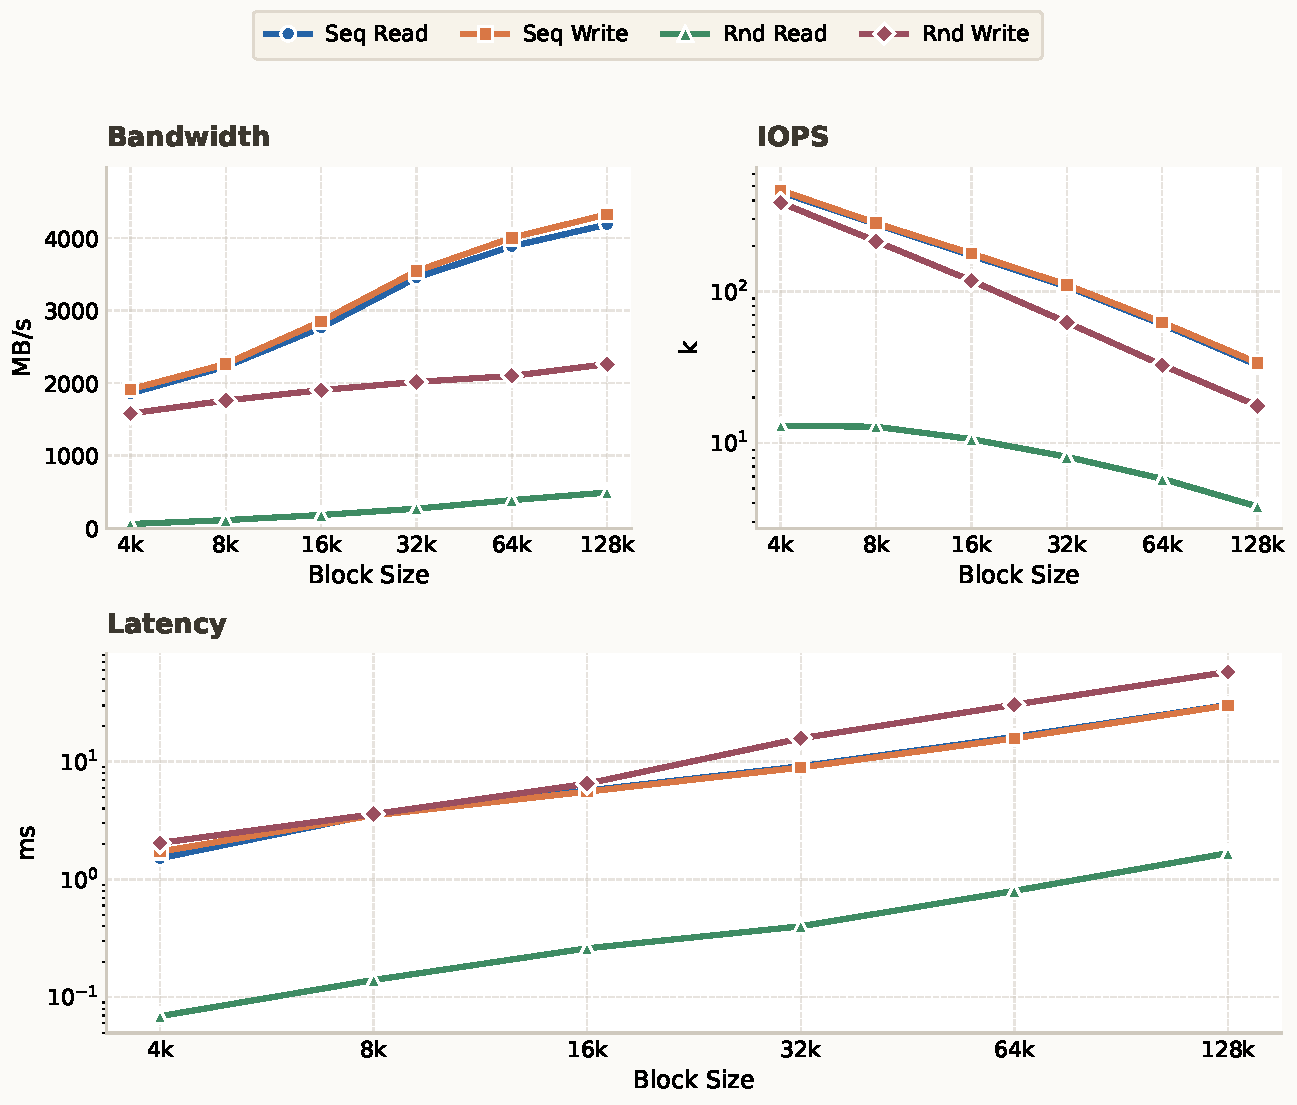
\includegraphics[width=0.98\linewidth,height=0.74\textheight,keepaspectratio]{images/chart_1.pdf}
  \caption{块大小（bs）对性能指标的影响（IOPS 与延迟子图采用对数坐标）}
  \label{fig:bs_all}
\end{figure}

% 结合数据与存储系统原理，块大小对性能的影响可以从以下角度理解：

\paragraph{块越大，带宽越容易上去}
顺序读写的带宽随着块大小增加持续上升，4k 时大约在 1.9 GB/s，128k 时分别达到 4189 MB/s 和 4330 MB/s。这个趋势比较直观：单次 I/O 搬运的数据更多，系统调用和请求组织的固定开销被摊薄了。随机读写的带宽也会上升，但斜率明显更缓，说明随机访问带来的额外开销并不会因为块变大就完全消失。

\paragraph{IOPS 和带宽呈现出明显的取舍关系}
块大小翻倍后，单次请求携带的数据也随之增加，所以虽然总带宽更高，但单位时间内能完成的 I/O 次数反而下降。这个现象在随机读上尤其明显，IOPS 从 13.0k 一路降到 3.8k。换句话说，如果应用更看重吞吐量，较大的块大小更合适；如果更在意操作次数和响应性，小块会更稳妥。

\paragraph{延迟曲线和前两项是一致的}
从图 \ref{fig:bs_all} 可以看到，块大小增大后，无论顺序还是随机，单次请求完成时间都在上升。顺序读写在 64k 之后增幅更明显，说明这时虽然带宽更高，但每个请求要等待更久。因此选择块大小时不能只盯着最高带宽，还要看业务能不能接受更长的单次响应时间。

\subsection{并发与队列深度（numjobs \& iodepth）的影响}

本组实验测试了 numjobs（1、4、8）和 iodepth（1、16、64）的不同组合，对四种读写模式（bs=4k, ioengine=pvsync）的影响。表 \ref{tab:concurrency_summary} 给出了关键汇总数据。

\begin{table}[H]
  \centering
  \renewcommand{\arraystretch}{1.25}
  \setlength{\tabcolsep}{10pt}
  \begin{tabular}{ccc cccc}
  \toprule
  \textbf{numjobs} & \textbf{iodepth} &
  \textbf{顺序读} & \textbf{顺序写} & \textbf{随机读} & \textbf{随机写} \\
  \midrule
  \multirow{3}{*}{1} & 1  & 1859 & 1915 & 57.2  & 1582 \\
                     & 16 & 1881 & 1885 & 71.7  & 1608 \\
                     & 64 & 1891 & 1885 & 68.5  & 1585 \\
  \midrule
  \multirow{3}{*}{4} & 1  & 2342 & 2402 & 858   & 546  \\
                     & 16 & 2400 & 2394 & 900   & 2124 \\
                     & 64 & 2418 & 2408 & 836   & 2108 \\
  \midrule
  \multirow{3}{*}{8} & 1  & 4527 & 2466 & 2717  & 1028 \\
                     & 16 & 3698 & 2488 & 2287  & 2168 \\
                     & 64 & 3368 & 2475 & 2279  & 2150 \\
  \bottomrule
  \end{tabular}
  \caption{并发数与队列深度对带宽的影响汇总（bs=4k，单位：MB/s）}
  \label{tab:concurrency_summary}
\end{table}

% 图 \ref{fig:iodepth_all} 展示了 iodepth 对性能的影响。

\begin{figure}[H]
  \centering
  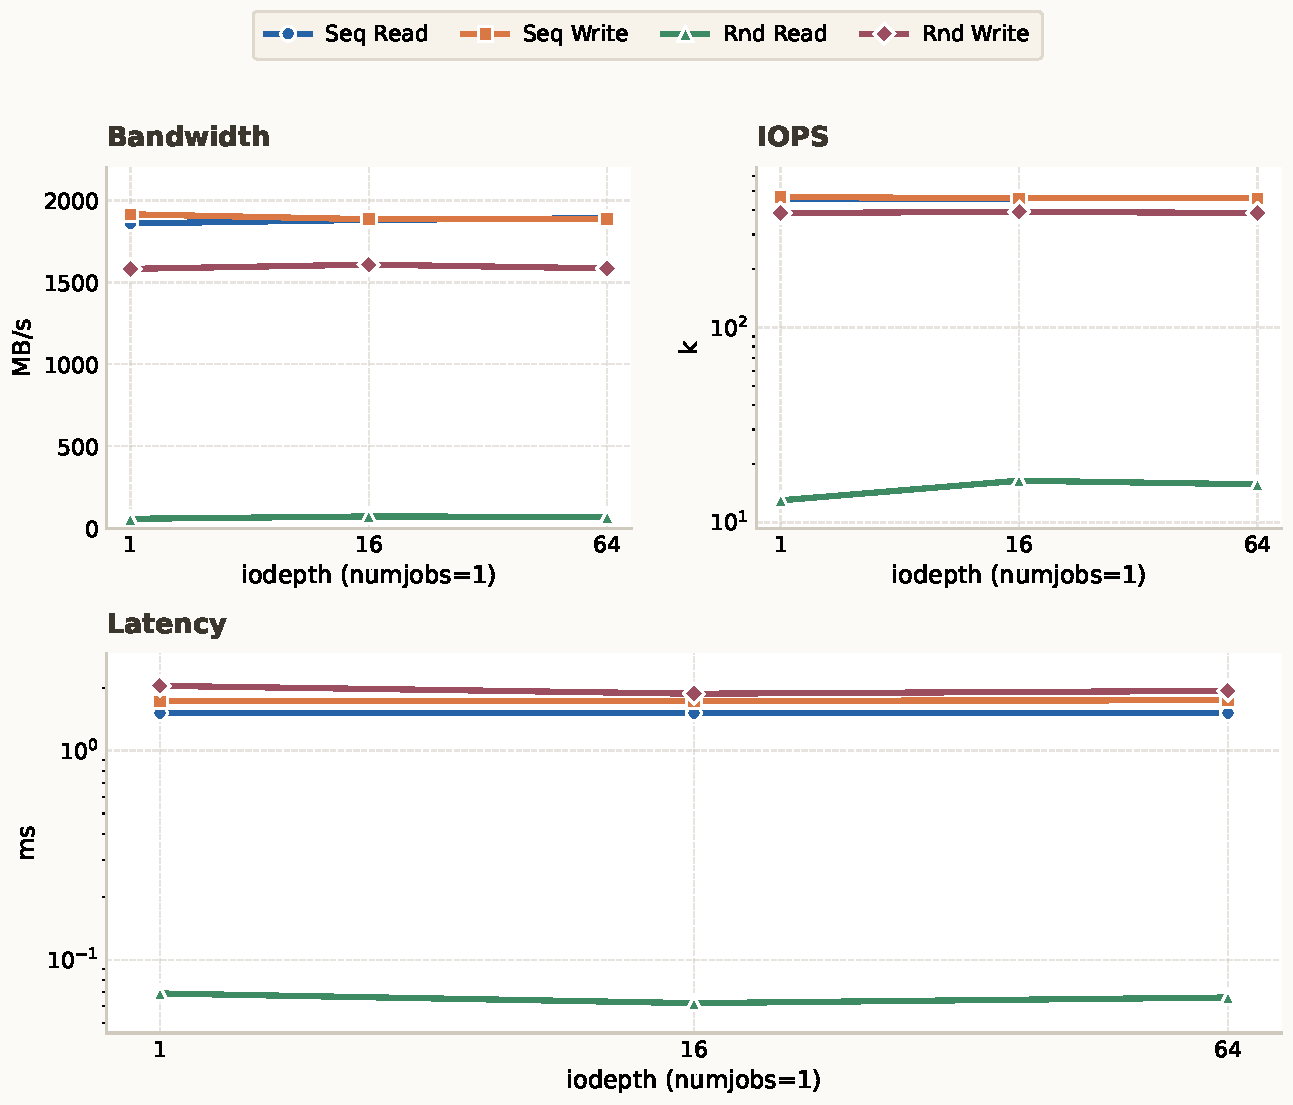
\includegraphics[width=0.98\linewidth,height=0.74\textheight,keepaspectratio]{images/chart_2.pdf}
  \caption{队列深度（iodepth）对性能指标的影响（IOPS 与延迟子图采用对数坐标）}
  \label{fig:iodepth_all}
\end{figure}

% 图 \ref{fig:iodepth_all} 分析如下（numjobs=1 固定，变化 iodepth）：

\paragraph{单线程下，iodepth 的作用并不明显}
在 \texttt{numjobs=1} 的条件下，把 \texttt{iodepth} 从 1 提高到 64，顺序读写带宽基本还停留在 1.88 GB/s 左右，随机写也没有明显变化。这个结果和本次使用的 \texttt{pvsync} 引擎有很大关系：它本质上还是同步 I/O，单线程里即使把队列深度参数设大，也很难像异步引擎那样真正挂起很多请求，所以曲线整体比较平。

\paragraph{随机读有小幅改善，但收益有限}
随机读带宽从 57.2 MB/s 提升到 71.7 MB/s，说明适当增加 \texttt{iodepth} 并不是完全没有帮助，只是收益不大。对这台机器和这组参数来说，单线程场景下真正限制性能的并不是“队列还不够深”，而是同步提交方式本身没有把并发度拉起来。

图 \ref{fig:numjobs_all} 展示了 numjobs 对性能的影响。

\begin{figure}[H]
  \centering
  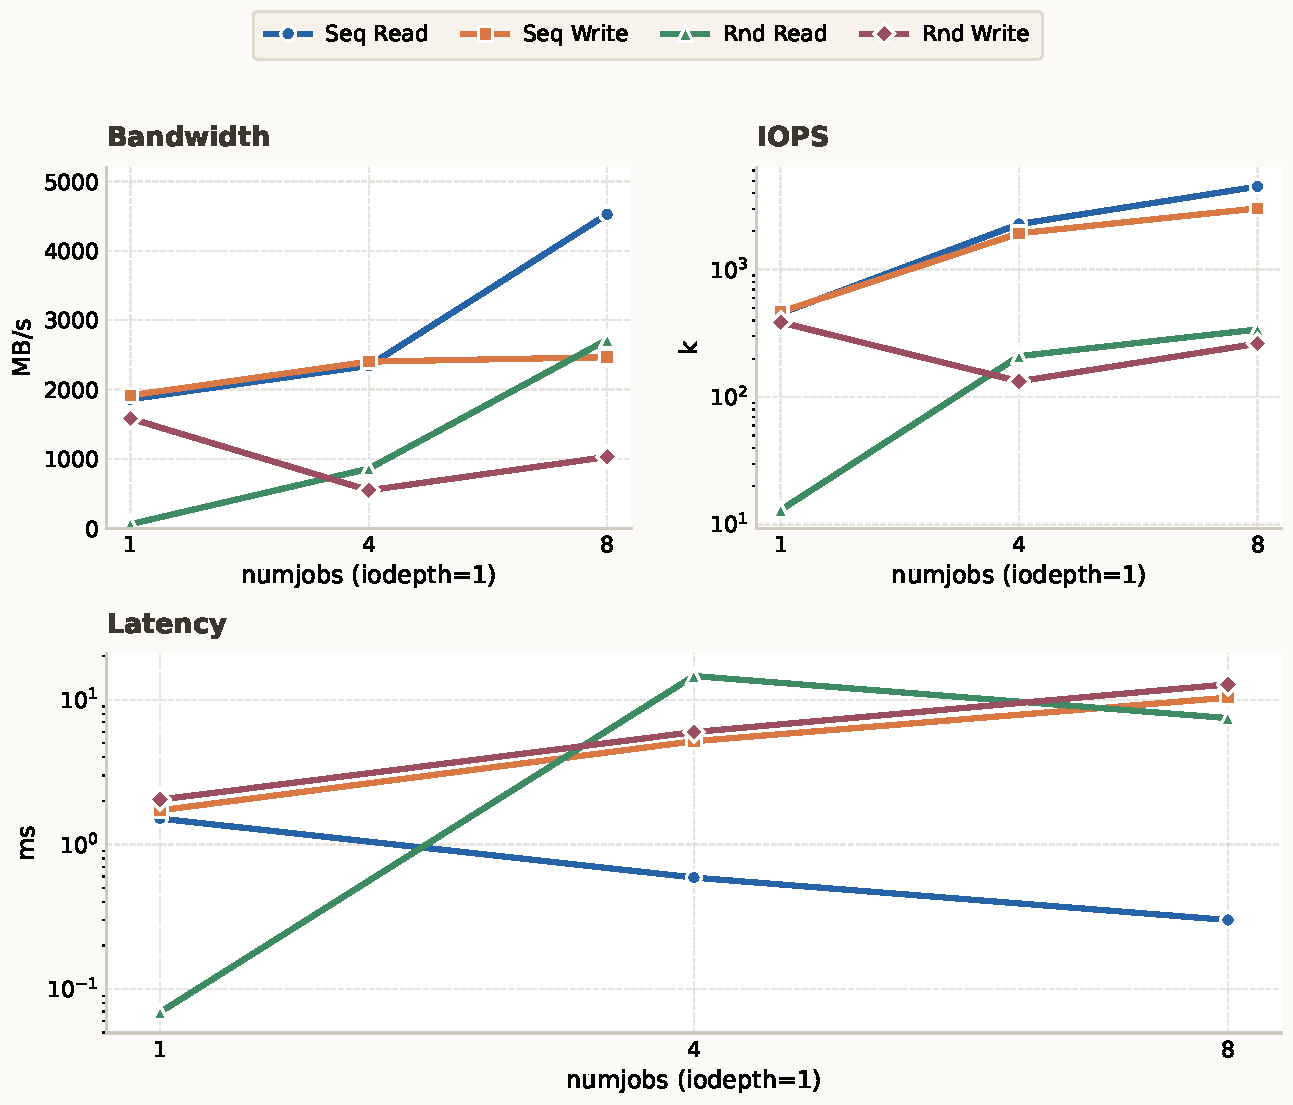
\includegraphics[width=0.98\linewidth,height=0.74\textheight,keepaspectratio]{images/chart_3.pdf}
  \caption{并发数（numjobs）对性能指标的影响（IOPS 与延迟子图采用对数坐标）}
  \label{fig:numjobs_all}
\end{figure}

图 \ref{fig:numjobs_all} 分析如下（iodepth=1 固定，变化 numjobs）：

\paragraph{\texttt{numjobs} 比 \texttt{iodepth} 更能把性能拉起来}
固定 \texttt{iodepth=1} 后，\texttt{numjobs} 从 1 增到 8，顺序读带宽从 1859 MB/s 提升到 4527 MB/s，随机读从 57.2 MB/s 提升到 2717 MB/s，变化非常明显。和上一小节对比可以看出，在 \texttt{pvsync} 这类同步引擎下，多开 worker 比单纯调大 \texttt{iodepth} 更有效，因为前者真的增加了同时发起 I/O 的线程数。

\paragraph{读负载的扩展性明显好于写负载}
顺序读和随机读在并发增加后都表现出较强的放大效应，尤其是随机读，增幅最为明显。这说明前面的基准测试里，随机读并不是“单次访问特别慢”，而是并发度太低，没有把 NVMe SSD 的并行能力吃满。随着 worker 数量增加，设备内部并行和操作系统调度都更容易被利用起来。

\paragraph{写场景的变化没有读那么规整}
顺序写在 \texttt{numjobs=4} 之后基本稳定在 2.4 GB/s 左右，随机写则出现了“先掉后升”的现象：1 job 时为 1582 MB/s，4 job 降到 546 MB/s，8 job 又回到 1028 MB/s。对这组文件级测试来说，写路径受到页缓存命中、后台回写时机以及设备内部整理的共同影响，所以波动会比读场景更大。也正因为如此，分析写入型负载时不能只看单个最高点，更要看整体趋势和稳定性。

\subsection{I/O 引擎（ioengine）对比}

本组实验对比了三种 I/O 引擎：pvsync（同步 POSIX I/O）、libaio（Linux 原生异步 I/O）、mmap（内存映射）在 bs=4k、numjobs=1、iodepth=1 条件下的性能表现。注意：由于测试环境不支持 io\_uring（运行时报错 ``io\_uring: cannot open shared object file''），该引擎未能测试。

表 \ref{tab:ioengine} 给出了各引擎在四种读写模式下的 IOPS、带宽与延迟数据，图 \ref{fig:ioengine_all} 以图表形式呈现了对比结果。

\begin{table}[H]
  \centering
  \renewcommand{\arraystretch}{1.25}
  \setlength{\tabcolsep}{10pt}
  \begin{tabular}{llccc}
  \toprule
  \textbf{引擎} & \textbf{测试类型} & \textbf{IOPS (k)} & \textbf{BW (MB/s)} & \textbf{延迟 (ms)} \\
  \midrule
  \multirow{4}{*}{pvsync}
      & 顺序读 & 279  & 1090 & 1.46 \\
      & 顺序写 & 450  & 1758 & 1.82 \\
      & 随机读 & 14.1 & 55.2 & 0.0678 \\
      & 随机写 & 371  & 1449 & 2.14 \\
  \midrule
  \multirow{4}{*}{libaio}
      & 顺序读 & 261  & 1020 & 1.55 \\
      & 顺序写 & 478  & 1868 & 1.72 \\
      & 随机读 & 15.7 & 61.2 & 0.0608 \\
      & 随机写 & 393  & 1534 & 2.03 \\
  \midrule
  \multirow{4}{*}{mmap}
      & 顺序读 & 257  & 1005 & 1.49 \\
      & 顺序写 & 422  & 1647 & 1.80 \\
      & 随机读 & 13.1 & 51.2 & 0.0733 \\
      & 随机写 & 12.5 & 48.8 & 0.0784 \\
  \bottomrule
  \end{tabular}
  \caption{I/O 引擎性能对比（bs=4k, numjobs=1, iodepth=1）}
  \label{tab:ioengine}
\end{table}

\begin{figure}[H]
  \centering
  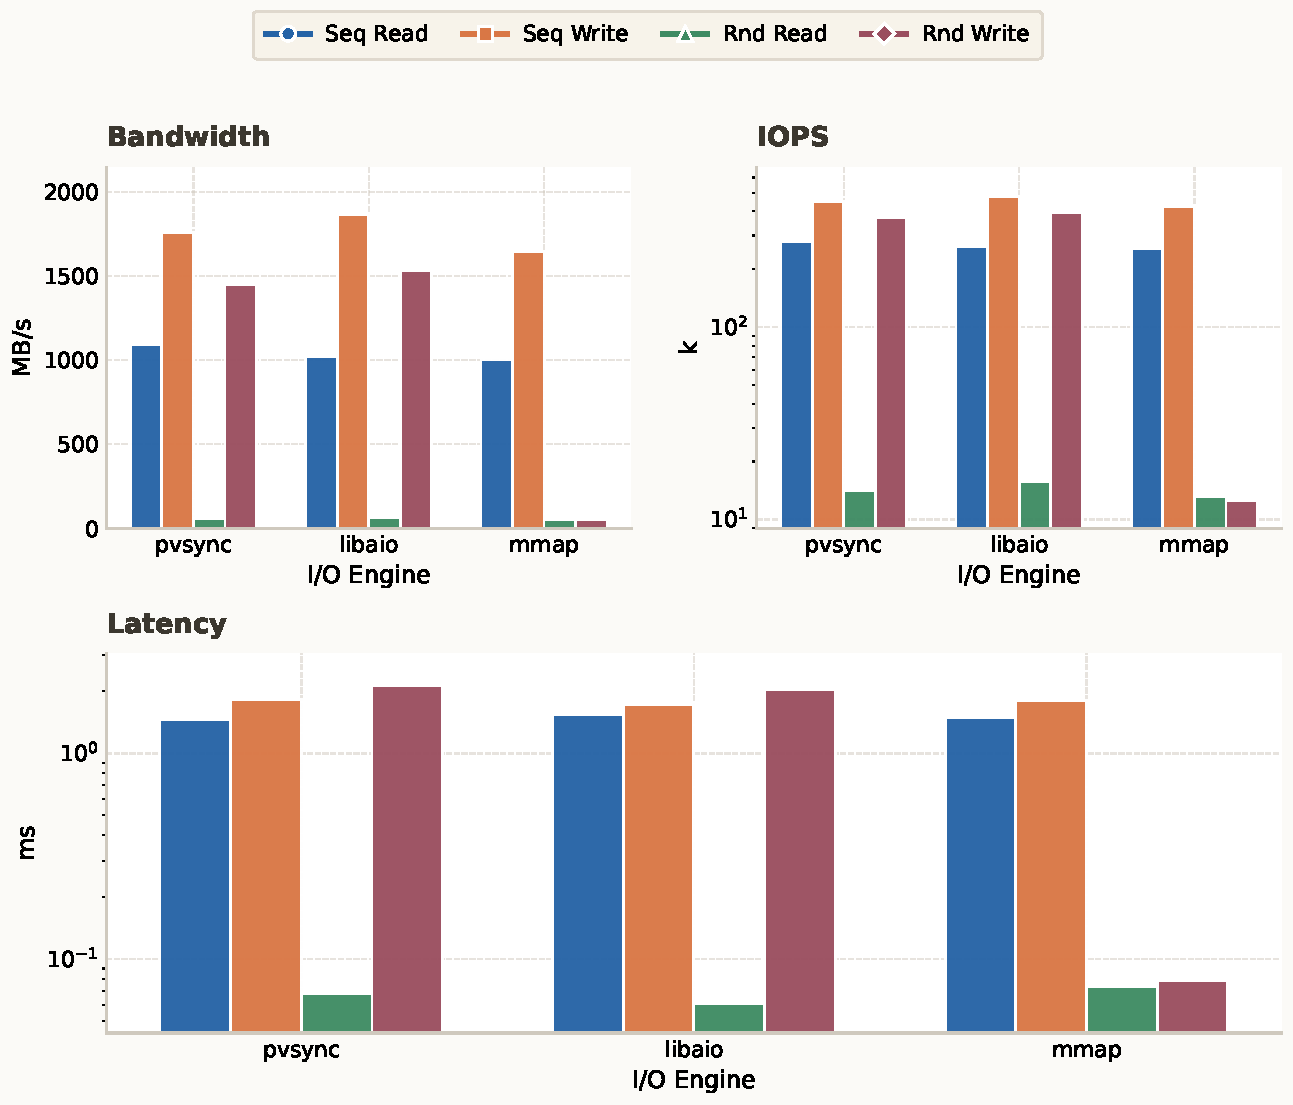
\includegraphics[width=0.98\linewidth,height=0.74\textheight,keepaspectratio]{images/chart_4.pdf}
  \caption{I/O 引擎（ioengine）对性能指标的影响（IOPS 与延迟子图采用对数坐标）}
  \label{fig:ioengine_all}
\end{figure}

图 \ref{fig:ioengine_all} 的分析如下：

\paragraph{\texttt{libaio} 略占优势，但不是压倒性差距}
在顺序读写和随机读这几组数据里，\texttt{libaio} 基本都比 \texttt{pvsync} 好一点，尤其是顺序写和随机写更明显一些；不过差距没有大到“换个引擎就翻倍”的程度。对这台 SSD 而言，在 4k、低并发的条件下，设备本身的能力仍然是主导因素，I/O 引擎更多是在细节上拉开差别。

\paragraph{\texttt{mmap} 不适合这组随机写测试}
\texttt{mmap} 在顺序读写上还能维持在同一量级，但一到随机写就直接掉到 12.5k IOPS、48.8 MB/s，和另外两个引擎拉开了一个数量级。这里更像是在测试页缓存和内存映射回写路径，而不是单纯测试块 I/O，所以它并不适合这种小块随机写场景。

\paragraph{关于 \texttt{io\_uring}}
这次环境里缺少相关共享库，所以没有拿到可用结果。为了避免空推测，本文不再对它的表现做展开，只保留“当前环境不支持测试”这一事实。

%---------------------------------------------------------------
\section{实验心得与总结}

这次实验最大的收获有两点。第一，\texttt{fio} 的结果一定要放回测试条件里理解：是否通过文件测试、是否经过页缓存、I/O 引擎是不是同步方式，这些都会直接改变最后看到的数字。第二，几组参数里最值得优先关注的是块大小和并发方式。块大小决定了吞吐和 IOPS 的取舍，而在这次 \texttt{pvsync} 测试里，真正把性能拉起来的是 \texttt{numjobs}，不是单纯把 \texttt{iodepth} 调大。

如果后续继续补实验，我会优先做两件事：一是加入 \texttt{direct=1}，尽量减小页缓存对结果的影响；二是把 \texttt{io\_uring} 补测出来，再和 \texttt{pvsync}/\texttt{libaio} 放在同一套参数下对比。这样得到的结论会比当前这份报告更完整，也更容易解释不同 I/O 路径之间的差别。

\newpage
\section{补充实验：Linux 与 Mac 基准对比}

为了观察相同 \texttt{fio} 参数在不同平台上的表现差异，我在一台 macOS 机器上补做了基础性能测试。Mac 侧仍然采用文件级测试，不直接访问裸设备，参数保持为 \texttt{size=5g}、\texttt{bs=4k}、\texttt{ioengine=pvsync}、\texttt{numjobs=1}、\texttt{iodepth=1}。四条基准命令已经整理到单独脚本 \texttt{run\_mac\_baseline.sh} 中，脚本会依次执行顺序读、顺序写、随机读、随机写，并将原始结果保存为 JSON 文件，便于后续复查。

\subsection{Mac 测试环境}

\begin{table}[H]
  \centering
  \renewcommand{\arraystretch}{1.25}
  \setlength{\tabcolsep}{10pt}
  \begin{tabular}{ll}
    \toprule
    \textbf{项目} & \textbf{配置说明} \\
    \midrule
    操作系统   & macOS 12.3.1 \\
    机器型号   & MacBook Pro (MacBookPro15,1) \\
    CPU 型号   & 6-Core Intel Core i7 2.2 GHz \\
    内存大小   & 16 GB \\
    存储设备   & APPLE SSD AP0256M 251 GB \\
    文件系统   & APFS \\
    fio 版本   & fio-3.39 \\
    测试文件   & 5 GB 普通文件 \\
    \bottomrule
  \end{tabular}
  \caption{补充实验的 Mac 测试环境}
  \label{tab:mac_env}
\end{table}

\subsection{基准结果对比}

\begin{table}[H]
  \centering
  \small
  \renewcommand{\arraystretch}{1.2}
  \setlength{\tabcolsep}{6pt}
  \begin{tabular}{lcccccc}
    \toprule
    \textbf{测试类型} & \textbf{Linux IOPS (k)} & \textbf{Mac IOPS (k)} & \textbf{Linux BW} & \textbf{Mac BW} & \textbf{Linux Lat} & \textbf{Mac Lat} \\
     &  &  & \textbf{(MB/s)} & \textbf{(MB/s)} & \textbf{(ms)} & \textbf{(ms)} \\
    \midrule
    顺序读 & 454.0 & 166.5 & 1859.0 & 682.0 & 1.51 & 0.0055 \\
    顺序写 & 467.0 & 100.6 & 1915.0 & 412.2 & 1.72 & 0.0093 \\
    随机读 & 13.0  & 28.6  & 57.2   & 117.1 & 0.069 & 0.0340 \\
    随机写 & 379.0 & 2.7   & 1553.0 & 11.1  & 2.04 & 0.3678 \\
    \bottomrule
  \end{tabular}
  \caption{Linux 主实验与 Mac 补充实验的基准结果对比}
  \label{tab:linux_mac_compare}
\end{table}

\begin{figure}[H]
  \centering
  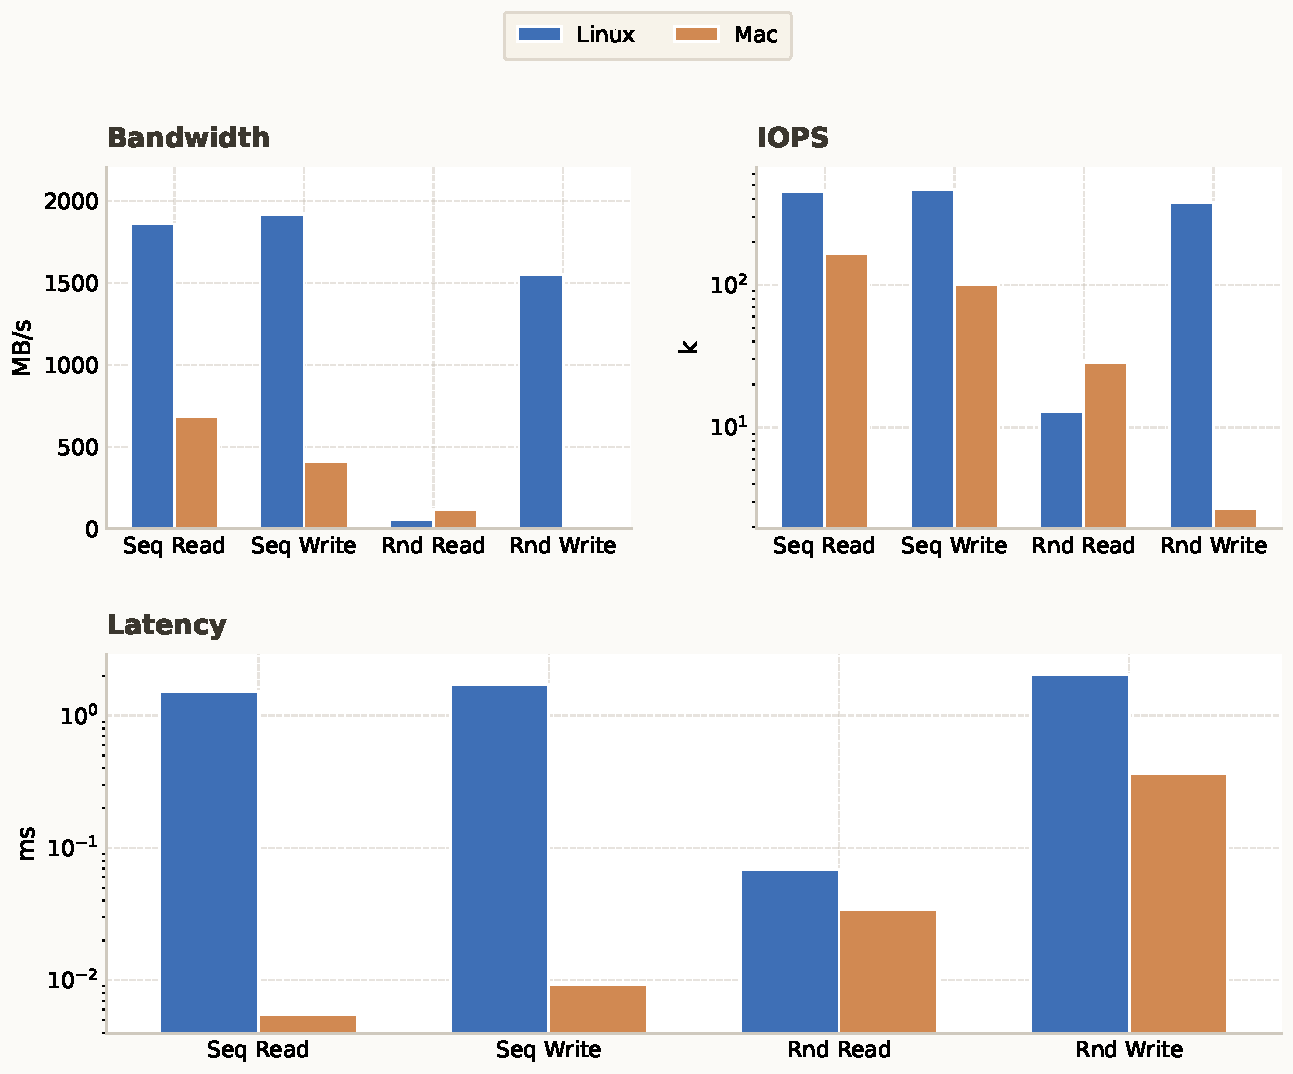
\includegraphics[width=0.98\linewidth,height=0.74\textheight,keepaspectratio]{images/chart_7.pdf}
  \caption{Linux 与 Mac 基准实验对比（Latency 子图采用对数坐标）}
  \label{fig:linux_mac_compare}
\end{figure}

从图 \ref{fig:linux_mac_compare} 和表 \ref{tab:linux_mac_compare} 可以看到，虽然两边的 \texttt{fio} 参数保持一致，但表现差异仍然非常明显。这说明文件级 I/O 测试的结果并不只取决于一条命令，还受到硬件代际、容量、文件系统实现、系统缓存以及磁盘剩余空间的共同影响。

\paragraph{顺序读写差距主要来自平台本身的上限不同}
Linux 主实验使用的是 Samsung 980 PRO 2TB，而补充实验中的 Mac 机器使用的是 2018 款 MacBook Pro 自带的 APPLE SSD AP0256M。两者在设备等级、容量和控制器能力上就不在一个量级上，因此顺序读写从一开始就存在明显差距。再加上 Mac 侧采用的是 APFS 文件系统，在 \texttt{pvsync + 单线程} 条件下，I/O 请求无法像高并发场景那样充分排队，最终顺序读只有约 682 MB/s，顺序写约 412 MB/s，明显低于 Linux 主实验。

\paragraph{随机读在 Mac 上更高，但这项结果要谨慎解读}
Mac 的随机读达到 28.6k IOPS、117.1 MB/s，反而高于 Linux 主实验中的 13.0k IOPS、57.2 MB/s。这里不能直接得出“Mac 随机读更强”的结论，因为两边测试的都是普通文件，而且都没有使用 \texttt{direct=1}。在这种条件下，随机读很容易受到页缓存、预读以及文件系统实现细节的影响。对 Mac 这台 16 GB 内存的机器而言，5 GB 测试文件完全有可能在前面的顺序读写之后留下较多缓存命中，因此这项数据更适合视为“文件级读路径”的表现，而不是裸设备随机读能力。

\paragraph{随机写差距极大，APFS 和剩余空间是关键因素}
真正拉开差距的是随机写。Mac 这组测试只有 2.7k IOPS、11.1 MB/s，而 Linux 主实验达到 379k IOPS、1553 MB/s。原因并不是某一个单点因素，而是几项条件叠加在一起：第一，APFS 本身是 Copy-on-Write 文件系统，小块随机写会频繁触发新块分配和元数据更新；第二，测试时 Mac 系统盘本身容量只有 251 GB，实验结束后可用空间只剩约 4.6 GiB，接近满盘状态，这会显著放大随机写时的空间管理和垃圾回收开销；第三，\texttt{pvsync} 在 \texttt{iodepth=1} 下几乎不给系统留出合并和隐藏延迟的机会，所以这些额外开销会直接反映到吞吐和延迟上。

\paragraph{延迟列可以参考，但不适合机械地逐项比较}
表中的 Mac 延迟整体都小于 Linux 主实验，尤其顺序读写只有微秒级。这说明在文件级同步 I/O 场景里，延迟指标对缓存状态非常敏感；同时，Linux 主实验中的延迟列取自正文基准表，本身就是在另一台机器、另一套文件系统环境里得到的。换句话说，这一列更适合帮助我们理解“哪类负载更容易受影响”，而不适合把两个平台的绝对值直接拿来判断谁更快。

综合来看，这组补充实验最有价值的地方不是给出一个“Mac 和 Linux 谁更强”的简单结论，而是说明：在相同 \texttt{fio} 参数下，平台差异、文件系统策略和剩余空间状态足以把结果拉开一个数量级。尤其是随机写场景，若不控制好文件系统类型、缓存和磁盘余量，测到的往往是整条 I/O 路径的综合行为，而不只是 SSD 芯片本身的性能。


%--------------------------人工智能使用情况说明--------------------------------
\newpage
\appendix
\section{人工智能使用情况说明}

本附录记录了我在完成本作业过程中的人工智能（AI）互动内容。以下是与 AI 的关键对话记录（由于多轮对话太多，篇幅太大，这里只放关键对话）：

\subsection{对话记录 1: 生成打印环境信息 `sh` 脚本}

\begin{tcolorbox}[colframe=blue!30!white, colback=blue!5!white, coltitle=black, title=对话内容]
\textbf{我:} 我需要测试环境说明，明确列出你的 CPU 型号、内存大小、操作系统版本、存储设备型号（如 HDD，SATA SSD，NVMe SSD 等），请帮我生成一个 `sh` 脚本，输出并写入一个 `.txt` 文件。

\textbf{AI:} 以下是一个 `sh` 脚本示例：
\begin{lstlisting}[breaklines=true, basicstyle=\ttfamily\small]
#!/bin/bash

# 输出到文件
output_file="system_info.txt"

# 获取 CPU 型号
cpu_model=$(lscpu | grep "Model name" | awk -F: '{print $2}' | sed 's/^[ \t]*//')

# 获取内存大小
memory_size=$(free -h | grep Mem | awk '{print $2}')

# 获取操作系统版本
os_version=$(cat /etc/os-release | grep 'PRETTY_NAME' | cut -d '=' -f2 | sed 's/"//g')

# 获取存储设备型号
storage_device=$(lsblk -d -o name,model | grep -i 'disk' | awk '{print $2}')

# 写入文件
echo "CPU 型号: $cpu_model" > $output_file
echo "内存大小: $memory_size" >> $output_file
echo "操作系统版本: $os_version" >> $output_file
echo "存储设备型号: $storage_device" >> $output_file

echo "环境信息已保存到 $output_file"
\end{lstlisting}
说明：
CPU 型号：使用 lscpu 命令提取 CPU 的型号。
内存大小：使用 free -h 命令提取总内存。
操作系统版本：读取 /etc/os-release 文件，提取操作系统版本信息。
存储设备型号：使用 lsblk 命令列出存储设备的型号。

运行该脚本后，系统环境信息将会被保存到 system\_info.txt 文件中。

你可以根据需要修改脚本输出的文件路径或者其他内容。如果需要进一步的调整，请告诉我！
\end{tcolorbox}


\subsection{对话记录 2: 生成人工智能使用情况说明章节 LaTeX 模板}

\begin{tcolorbox}[colframe=blue!30!white, colback=blue!5!white, coltitle=black, title=对话内容]
\textbf{我:} 我需要生成一个关于人工智能使用情况说明的 LaTeX 模板，要求格式美观。我只需要放对话内容，不需要分析

\textbf{AI:} 明白了！如果你只需要放置与 AI 的对话内容而不进行分析，下面是一个简洁的 LaTeX 格式，专门用于展示你与 AI 的对话记录。这部分内容可以放在附录中，并确保每次与 AI 的对话都清晰可见。
\begin{lstlisting}[breaklines=true, basicstyle=\ttfamily\small]
%--------------------------人工智能使用情况说明--------------------------------
\appendix
\section{人工智能使用情况说明}

本附录记录了我在完成本作业过程中的人工智能（AI）互动内容。以下是与 AI 的对话记录：

\subsection{对话记录 1: 生成 `sh` 脚本}

\textbf{我:} 我需要测试环境说明，明确列出你的 CPU 型号、内存大小、操作系统版本、存储设备型号（如 HDD，SATA SSD，NVMe SSD 等），请帮我生成一个 `sh` 脚本，输出并写入一个 `.txt` 文件。

\textbf{AI:} 以下是一个 `sh` 脚本示例：

\begin{verbatim}
（略）
\textbackslash end\{verbatim\}

\subsection{对话记录 2: 生成 LaTeX 模板}

（略）

% 可以继续添加更多的对话记录
\end{lstlisting}

说明：
每段对话：每次与你和 AI 的对话都以 \subsection{对话记录 X} 来组织，使其清晰区分。
格式：使用 \textbf\{\} 来突出显示提问和 AI 的回答，并且 \verb|\begin{verbatim}...\end{verbatim}| 用于展示代码或命令行内容，确保其原始格式不变。
结构清晰：对话内容按顺序排列，确保在附录中可以直接查看完整的对话记录。

你可以继续在这个模板中添加更多的对话记录。希望这样满足你的需求！如果有任何其他的格式要求或细节修改，随时告诉我！
\end{tcolorbox}


% 可以继续添加更多的对话记录
\subsection{对话记录 3: 润色报告图表与正文表述}

\begin{tcolorbox}[colframe=blue!30!white, colback=blue!5!white, coltitle=black, title=对话内容]
\textbf{我:} 我现在希望你把我的报告变得好看一点，主要是修改图表，现在的图表太小而且很丑。你可以修改配色和作图形式吗？另外第四章节有点 AI 写作的风格太重了，帮我改一下。

\textbf{AI:} 可以。我建议把原来横向排成一行的 1x3 小图改成更大的分层布局：上面放带宽和 IOPS，下面单独放延迟，这样每张图在 A4 页面里会更舒展，图例也更清楚。配色方面我会换成更稳一点的蓝、橙、绿、暗红组合，避免颜色过亮。正文部分则不再用空泛总结，而是尽量贴近你这次实验的真实现象，比如指出文件级测试会受页缓存和文件系统行为影响，以及哪些结论更适合解释“趋势”，哪些不能直接当作设备极限。

\textbf{我:} 好，那就按这个思路改。图表和正文都要统一风格。

\textbf{AI:} 明白。我会同时修改作图脚本和 LaTeX 插图尺寸，然后把第四章和总结部分改成更像实验记录的写法，而不是模板式表述。
\end{tcolorbox}

\subsection{对话记录 4: 生成 Mac 基准测试脚本}

\begin{tcolorbox}[colframe=blue!30!white, colback=blue!5!white, coltitle=black, title=对话内容]
\textbf{我:} 我想补充一个实验，就是在 Mac 上面的实验，可以只补基准实验。你先帮我跑实验结果，需要有 sh 文件脚本，实验结果还要整理成 md。

\textbf{AI:} 可以。我会先确认 Mac 侧的系统环境和 \texttt{fio} 是否可用，再把四条基准测试命令单独写进一个 \texttt{run\_mac\_baseline.sh} 脚本里，保持和 Linux 基准一致的参数：\texttt{size=5g}、\texttt{bs=4k}、\texttt{ioengine=pvsync}、\texttt{numjobs=1}、\texttt{iodepth=1}。脚本会先记录 macOS 版本、CPU、内存和 SSD 信息，再依次运行顺序读、顺序写、随机读、随机写，并把原始结果保存成 JSON，最后再整理成一份 Markdown 说明。

\textbf{我:} 要求用 5G 的，和 Linux 的基准测试环境一样。然后把 fio 的命令写入一个 sh 文件里面。

\textbf{AI:} 好，我会把脚本改成显式的四条 \texttt{fio} 命令，不用循环隐藏参数；默认文件大小就是 \texttt{5g}，这样脚本内容和报告里的基准命令能直接对应起来。
\end{tcolorbox}

\subsection{对话记录 5: 辅助分析 Linux 与 Mac 的差异}

\begin{tcolorbox}[colframe=blue!30!white, colback=blue!5!white, coltitle=black, title=对话内容]
\textbf{我:} 我想在实验总结之后新开一页，然后新开一个章节叫补充实验，把这两个基准测试的对比放在里面。你可以尝试画图可视化和画表格可视化，然后分析差异，为什么 Mac 差别这么大，而且同时要把 Mac 的环境列出来。

\textbf{AI:} 可以。我会新加一张 Linux 和 Mac 基准结果的对比图，再配一张总表，把 IOPS、带宽和延迟放在同一页里集中展示。分析时我会重点解释三件事：第一，两台机器的 SSD 本身就不在一个等级上；第二，Mac 侧使用 APFS，随机小块写入会受到 Copy-on-Write 和元数据更新影响；第三，文件级同步 I/O 测试本身会受到缓存和剩余空间状态影响，所以结果反映的是“整条 I/O 路径”的综合行为，而不只是 SSD 芯片本身。

\textbf{我:} 那就按这个方向写，不要写得太空，要能看出是结合数据分析出来的。

\textbf{AI:} 明白。我会把分析尽量和表里的具体数值对应起来，比如顺序读写为什么都比 Linux 低、为什么 Mac 随机读反而更高、以及为什么随机写在 Mac 上只有很低的吞吐，并把这些现象和 APFS、缓存、剩余空间联系起来解释。
\end{tcolorbox}

\end{document}
